%! TEX root = main.tex

\chapter{Sound Radiation}

This chapter focuses on the radiation of sound from vibrating sources into an unbounded acoustic medium. The objective is to relate the source motion to the radiated pressure field and to quantify how efficiently acoustic power is transferred to the surrounding air. We start from elementary source models, which provide useful scaling laws with frequency and clarify the role of directivity in the radiated field. 

\section{Simple Multipole Sources}

\subsection{Monopole Source} 

A monopole can be modeled as a small spherical source of radius \( a \) pulsating at angular frequency \( \omega \). Its acoustic volume flow is
\[
Q = 4\pi a^{2} v(a)
\]
where \( v(a) \) is the normal velocity at the source surface. For \( ka \ll 1 \), the pressure at distance \( r \) from the source is
\[
p(r) = \frac{j\omega\rho}{4\pi r} Q e^{-jkr}
\]
The radiated acoustic power is obtained from the intensity integrated over a spherical surface \( S \)
\[
P = \int_{S}\frac{p^{2}}{\rho c} dS = \frac{\omega^{2}\rho Q^{2}}{8\pi c}
\]
Therefore the radiated power scales with \( \omega^{2} \). 

\subsection{Dipole Source} 

\begin{figure}[!htb]
    \centering
    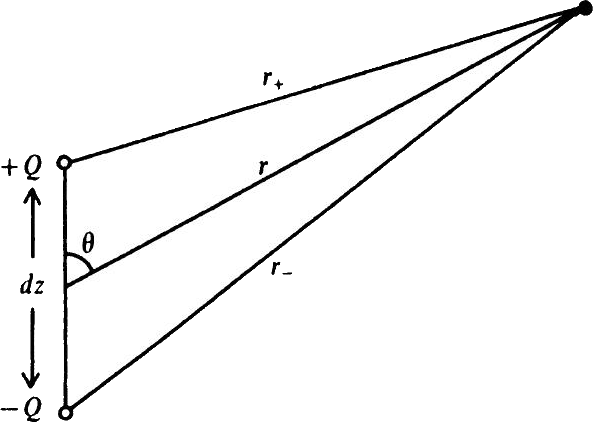
\includegraphics[width=0.6\linewidth]{00_Images/05_chapter/01.png}
    \caption{Dipole geometry and observation angle \(\theta\)}
    \label{fig:dipole_geom}
\end{figure}

A dipole is defined as two spherical sources of strength \( \pm Q \) separated by a distance \( dz \) that tends to zero. The pressure at \( (r,\theta) \) can be written as following, figure \ref{fig:dipole_geom} summarizes the geometry.
\[
p(r,\theta) = \frac{j\omega\rho}{4\pi}\left(\frac{e^{-jkr_{+}}}{r_{+}} - \frac{e^{-jkr_{-}}}{r_{-}}\right)Q
\]
If \( dz \to 0 \) and \( Q \to \infty \) while keeping \( \mu = Qdz \) finite, one obtains
\[
p(r,\theta) = \frac{\omega^{2}\rho}{4\pi c r}\left(1 + \frac{1}{jkr}\right)e^{-jkr}\mu\cos\theta
\]
The corresponding radiated power is
\[
P = \frac{\omega^{4}\rho\mu^{2}}{24\pi c^{3}}
\]
showing a \( \omega^{4} \) dependence, which makes dipole radiation much less efficient than monopole radiation at low frequencies.

\subsection{Quadripole Source} 

A quadripole field can be generated by combining dipole sources, as shown in figure \ref{fig:quadrupole_geom}, leading to a pressure of the form
\[
p_{q} = -jk^{3}\left(\frac{\rho c Q dz dx}{4\pi r}\right)\cos(\vv{r},\mathbf{z})\cos(\vv{r},\mathbf{x})e^{-jkr}
\]

\begin{figure}[!htb]
    \centering
    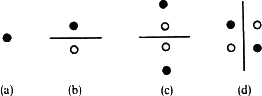
\includegraphics[width=0.8\linewidth]{00_Images/05_chapter/02.png}
    \caption{Quadrupole source as a combination of dipoles}
    \label{fig:quadrupole_geom}
\end{figure}

As the source order increases, the angular dependence becomes more complex and the low-frequency radiation efficiency decreases markedly compared to lower-order sources.

\section{Distribution of Point Sources}

The radiation pattern of an extended source can be understood by combining elementary point-like radiators with prescribed relative phases. In the following, \( Q \) denotes the acoustic volume flow associated with each point source and \( r \) is the distance to the observation point, with \( r \gg d \).

\subsection{Two Point-Like Sources} 

\begin{figure}[!htb]
    \centering
    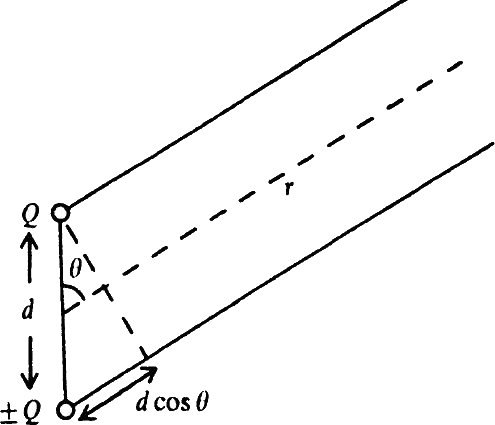
\includegraphics[width=0.5\linewidth]{00_Images/05_chapter/03.png}
    \caption{Geometry for two point-like sources separated by \(d\)}
    \label{fig:two_sources_geom}
\end{figure}

Consider two sources separated by a distance \( d \) and an angle \( \theta \), as illustrated in figure \ref{fig:two_sources_geom}. In the far field, the pressure can be approximated as
\[
p \approx \left(\frac{j\omega\rho Q}{4\pi r}\right)e^{-jkr}\left(e^{\frac{1}{2}jkd\cos\theta} \pm e^{-\frac{1}{2}jkd\cos\theta}\right)
\]
where the sign \( + \) corresponds to in-phase sources, while \( - \) corresponds to opposite-sign sources. The interference term introduces strong angular variations as \( kd \) increases. The radiated power is
\[
P = \frac{\omega^{2}\rho Q^{2}}{4\pi c}\left(1 \pm \frac{\sin(kd)}{kd}\right)^{2}
\]
Three limiting regimes are of interest. If \( kd \simeq 1 \), the pressure tends to vanish for several angles \( \theta \). If \( kd \ll 1 \), the power goes to zero for opposite-sign sources, while it becomes four times the power of a single monopole with strength \( Q \) in the in-phase case. If \( kd \gg 1 \), the power converges to twice the monopole power. The dependence of the radiated power on the non-dimensional spacing \(kd\) is shown in figure \ref{fig:two_sources_interf}.

\begin{figure}[!htb]
    \centering
    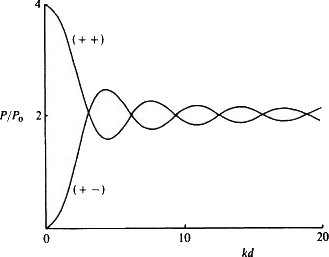
\includegraphics[width=0.6\linewidth]{00_Images/05_chapter/04.png}
    \caption{Interference effects for two point sources as a function of \(kd\)}
    \label{fig:two_sources_interf}
\end{figure}

\subsection{Line of 2N Sources} 

Consider a linear distribution of \( 2N \) sources at spacing \( d \), either all in phase or with alternating signs. The far-field pressure can be written as
\[
p_{\pm} \approx \frac{j\omega\rho Q}{4\pi r}e^{-jkr}\sum_{n=1}^{N}\pm(-1)^{n}\left[e^{(n-\frac{1}{2})jkd\cos\theta} \pm e^{(-n-\frac{1}{2})jkd\cos\theta}\right]
\]
For a co-phase array the expression reduces to
\[
p_{+} \approx \frac{j\omega\rho Q}{4\pi r}e^{-jkr}\frac{\sin(Nkd\cos\theta)}{\sin\left(\frac{1}{2}kd\cos\theta\right)}
\]
At broadside, \( \theta = 90^{\circ} \), the pressure tends to that of a single point source of strength \( 2NQ \) placed at the array center. The main lobe width scales as \( 2\pi/(Nkd) \). If \( d > \lambda/2 \), additional maxima appear at angles \( \theta^{\ast} = \cos^{-1}(2n\pi/(kd)) \). At high frequency the total radiated power is \( NP_{0} \), while at low frequency it is \( N^{2}P_{0} \), with \( P_{0} \) the power of one source.

\subsection{Antiphase Array} 

For alternating signs, the pressure can be written as
\[
p_{-}(r,\theta,t) \approx \left(\frac{j\omega\rho Q}{4\pi r}\right)e^{-jkr}\sum_{n=1}^{N}(-1)^{n}2j\sin\left(\left(n-\frac{1}{2}\right)kd\cos\theta\right)e^{j\omega t}
\]
or equivalently
\[
p_{-}(r,\theta,t) \approx \left(\frac{j\omega\rho Q}{4\pi r}\right)e^{-jkr}\left[\frac{(-1)^{N}\sin(Nkd\cos\theta)}{\cos\left(\frac{1}{2}kd\cos\theta\right)}\right]e^{j\omega t}
\]
An antiphase array is less efficient because the acoustic flow tends to remain internal to the array, reducing the energy escaping to the far field. At low frequency, \( \lambda > 2d \), the radiation efficiency approaches that of a single monopole source. At high frequency, \( \lambda < 2d \), maxima occur at \( \theta^{\ast} = \cos^{-1}((2n-1)\pi/(kd)) \). The evolution of the radiation pattern with the number of sources and with phase relation is illustrated in figure \ref{fig:line_arrays}.

\begin{figure}[!htb]
    \centering
    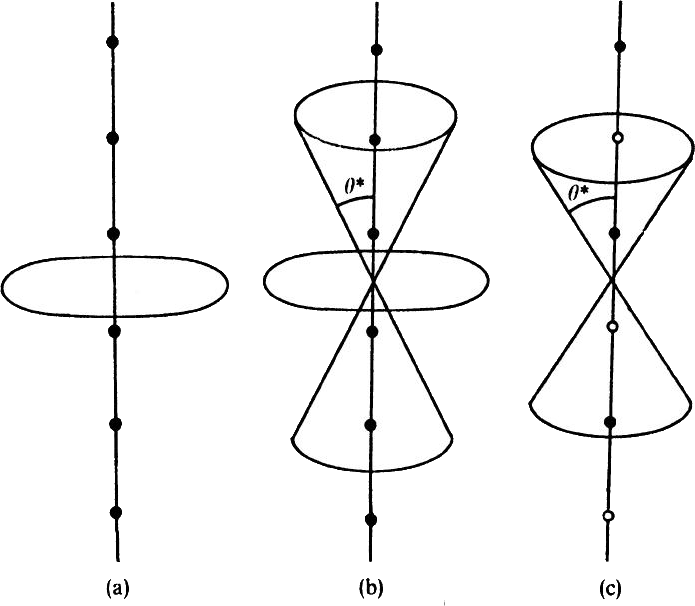
\includegraphics[width=0.6\linewidth]{00_Images/05_chapter/05.png}
    \caption{Radiation patterns of line arrays (in-phase and antiphase cases)}
    \label{fig:line_arrays}
\end{figure}

\section{Radiation from a Spherical Source}

In the previous discussion the radiating element was assumed to be acoustically compact, namely \( ka \ll 1 \). We now remove this constraint and consider a pulsating sphere of radius \( a \), whose normal surface velocity is \( u e^{j\omega t} \). The acoustic pressure at distance \( r \) from the center can be written as
\[
p(r,t) = j c \rho \frac{a^{2} k u}{r}\left(\frac{1 - jka}{1 + k^{2}a^{2}}\right)e^{-jk(r-a)}e^{j\omega t}
\]
The total radiated power follows from integrating the intensity over a spherical surface
\[
P = 2\pi \rho c \frac{k^{2}a^{4}u^{2}}{1 + k^{2}a^{2}}
\]
Two limiting cases clarify the frequency dependence. For \( ka \gg 1 \),
\[
P = 2\pi \rho c a^{2}u^{2}
\]
so the radiated power no longer increases with frequency. For \( ka \ll 1 \),
\[
P = 2\pi \rho c (ka)^{2} a^{2}u^{2}
\]
therefore the radiated power increases with frequency. Since most musical instruments operate with \( ka < 1 \), increasing the effective size of the radiating surface is advantageous at low frequency. The acoustic field exerts a mechanical load on the source surface. Let \( S = 4\pi a^{2} \) be the sphere area. The resulting force is
\[
F = 4\pi a^{2}p(a)
\]
and it can be expressed as
\[
F = \left(\rho c S \frac{k^{2}a^{2}}{1 + k^{2}a^{2}} + j\rho c S \frac{ka}{1 + k^{2}a^{2}}\right)u = (R_{m} + jX_{m})u
\]
The term \( R_{m}u \) represents the dissipative radiation load. It increases as \( (ka)^{2} \) at low frequency and then saturates. The term \( X_{m}u \) represents the mass load associated with the co-moving air. It grows approximately as \( ka \) for \( ka < 1 \) and then decreases as \( (ka)^{-1} \) for \( ka > 1 \). As a consequence, \( X_{m}u \) dominates at low frequency, whereas \( R_{m}u \) dominates at high frequency. Typical trends of the radiation resistance \(R_m\) and reactance \(X_m\) for a pulsating sphere are shown in figure \ref{fig:sphere_load}.

\begin{figure}[!htb]
    \centering
    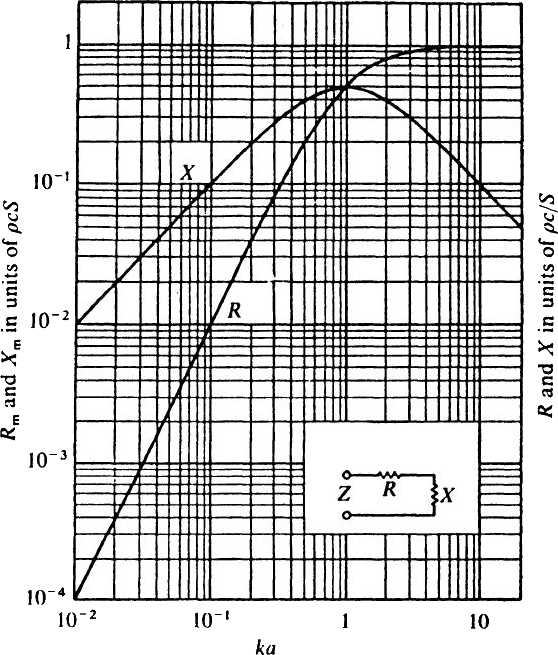
\includegraphics[width=0.5\linewidth]{00_Images/05_chapter/06.png}
    \caption{Radiation resistance and reactance of a pulsating sphere versus \(ka\)}
    \label{fig:sphere_load}
\end{figure}


\section{Strings as an Extreme Case of Line Sources}

Linear radiators provide a useful model for vibrating strings. We consider a cylindrical source of radius \( a \) oscillating at angular frequency \( \omega \), and we assume a small radius such that \( ka \ll 1 \). Let \( u e^{j\omega t} \) be the vibration velocity. In the far field, the acoustic intensity at distance \( r \) takes the form
\[
I \approx \left(\frac{\pi \rho \omega^{3} a^{2} u^{2}}{4 c^{2} r}\right)\cos^{2}\phi
\]
where \( \phi \) is the observation angle with respect to the source axis. The total radiated power is then
\[
P \approx \frac{\rho \pi^{2} \omega^{2} a^{4} u^{2}}{4 c^{2}}
\]
This expression shows a very strong dependence on both \( \omega \) and \( a \). In particular, for the strings encountered in musical instruments the radius is extremely small, and the resulting radiated power is therefore negligible compared to the radiation from larger vibrating surfaces. 

\section{Radiation from Baffled Plane Sources}

\begin{figure}[!htb]
    \centering
    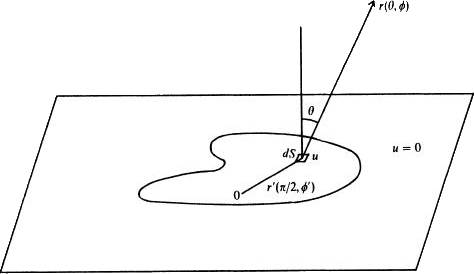
\includegraphics[width=0.7\linewidth]{00_Images/05_chapter/07.png}
    \caption{Geometry for radiation from a baffled plane source (Rayleigh integral)}
    \label{fig:rayleigh_geom}
\end{figure}

A widely used idealization for vibrating plates and membranes is a plane source mounted in an infinite rigid baffle. The source surface is described by coordinates \( \vv{r}' \), while the acoustic pressure is evaluated at an observation point \( \vv{r} \) with \( |\vv{r}| \gg |\vv{r}'| \) (the geometry is shown in figure \ref{fig:rayleigh_geom}). The infinitesimal contribution of a surface element \( dS \) vibrating with normal velocity \( u(\vv{r}') \) is
\[
dp(\vv{r}) = \frac{j\omega\rho}{2\pi r} e^{-jk|\vv{r}-\vv{r}'|} u(\vv{r}') dS
\]
Integrating over the entire radiating surface \( S \) yields, in the far field,
\[
p(r,\theta,\phi) = \frac{j\omega\rho}{2\pi r} e^{-jkr} \iint_{S} e^{jkr'\sin\theta\cos(\phi-\phi')} u(r') r' d\phi' dr'
\]
The pressure field is therefore proportional to the spatial Fourier transform of the surface velocity distribution.

\subsection{Circular Piston} 

Consider a circular piston of radius \( a \) vibrating with uniform normal velocity \( u \). The far-field pressure can be written as
\[
p \approx \frac{1}{2} j\omega\rho u a^{2} \frac{e^{-jkr}}{r}\left[\frac{2J_{1}(ka\sin\theta)}{ka\sin\theta}\right]
\]
For \( ka \ll 1 \) the directivity factor tends to one and
\[
p \approx \frac{1}{2} j\omega\rho u a^{2} \frac{e^{-jkr}}{r}
\]
so the source is approximately isotropic. As frequency increases, the first zero of \( J_{1} \) implies a radiation null at
\[
\theta^{\ast} = \sin^{-1}\left(\frac{3.83}{ka}\right)
\]
highlighting the progressive narrowing of the main lobe.

\subsection{Non-uniform Velocity Distributions} 

If the velocity is not constant over the surface, as for membranes vibrating in higher modes, nodal lines and nodal circles imply regions of opposite sign. A cross flow is required to sustain these patterns, and the associated cancellation makes such modes inefficient radiators, similarly to arrays with alternating signs. The most effective membrane modes are the axisymmetric ones, which have a monopole rather than a dipole character. 

\subsection{Mechanical Load on the Piston} 

The acoustic field exerts a load on the source that can be written as
\[
F = (R_{m} + jX_{m})u = \rho c S u (A + jB)
\]
where \( S \) is the piston area. The coefficients are
\[
A = 1 - \frac{J_{1}(2ka)}{ka}
\]
\[
B = \frac{H_{1}(2ka)}{ka}
\]
with \( J_{1} \) the Bessel function and \( H_{1} \) the Struve function. Their limiting behaviors are
\[
A \to \frac{1}{2}(ka)^{2} \quad ka \ll 1
\]
\[
A \to 1 \quad ka \gg 1
\]
\[
B \to \frac{8ka}{3\pi} \quad ka \ll 1
\]
\[
B \to \frac{2}{\pi ka} \quad ka \gg 1
\]
These trends are consistent with the frequency dependence previously observed for the mechanical radiation load of a pulsating sphere. 

\section{Unbaffled Radiators}

Only a limited number of musical instruments can be idealized as sources mounted in an infinite rigid baffle. In practice, most radiating surfaces are unbaffled, and therefore radiate into the full space, over a solid angle \( 4\pi \) rather than \( 2\pi \). A direct consequence concerns the radiated power at low frequency. When \( ka < 1 \), the absence of the baffle reduces the radiated power by approximately a factor \( 2 \) compared to the baffled case. At high frequency, the directional behavior is essentially unchanged with respect to a baffled radiator. As a result, the spectrum of the radiated signal from an unbaffled source is shifted towards higher frequencies compared to the baffled case. A useful characterization is provided by the mechanical radiation resistance of an unbaffled piston. In the low-frequency range, for \( ka < 2 \),
\[
R_{m} \approx 3 \times 10^{-2}\rho c S (ka)^{4}
\]
while for \( ka > 3 \),
\[
R_{m} \approx \rho c S
\]
In the regime \( ka < 2 \), most of the radiation is suppressed, consistently with the strong reduction of radiated power for unbaffled sources at low frequency. 

\section{Radiation from Large Plates}

Consider a large plate supporting a bending wave that propagates along the \( x \) direction. The normal particle velocity on the plate surface can be written as
\[
u(x) = u_{p} e^{-j k_{p} x}
\]
where \( k_{p} = \omega / v_{p} \) and \( v_{p} \) is the phase velocity of the plate wave. Let \( (x,z) \) denote a point in the surrounding air. Assuming a plane wave field in air, the acoustic pressure can be expressed as
\[
p(x,z) = \rho c u_{A}(x,z)
\]
with
\[
u_{A}(x,z) = A e^{-j(k_{x}x + k_{z}z)}
\]
Imposing the boundary condition at the plate surface, \( u_{A}(x,0) = u(x) \), yields \( k_{x} = k_{p} \) and \( A = u_{p} \). The remaining component follows from the dispersion relation in air
\[
k_{z}^{2} = \frac{\omega^{2}}{c^{2}} - k_{x}^{2} = \omega^{2}\left(\frac{1}{c^{2}} - \frac{1}{v_{p}^{2}}\right)
\]
Two regimes arise depending on the relative magnitude of \( v_{p} \) and \( c \). If \( v_{p} > c \), then \( k_{z} \) is real and the field propagates away from the plate. The decomposition of the acoustic wavevector into tangential and normal components, and the associated radiation angle, are illustrated in figure \ref{fig:plate_radiation_angle}. The propagation direction can be written as
\[
\tan\theta = \frac{k_{z}}{k_{x}} = \left(\frac{v_{p}^{2}}{c^{2}} - 1\right)^{1/2}
\]
If instead \( v_{p} < c \), then \( k_{z} \) is imaginary and the acoustic field decays exponentially with \( z \), corresponding to an evanescent wave. For bending waves in plates, the phase velocity increases with frequency. As a consequence, there exists a frequency above which \( v_{p} > c \) and efficient radiation becomes possible. For complex surface motion, only the high-frequency components satisfy this condition and can propagate in air. When the plate is finite rather than infinite, the transition is less sharp and some radiation contributions may still be observable at low frequency.

\begin{figure}[!htb]
    \centering
    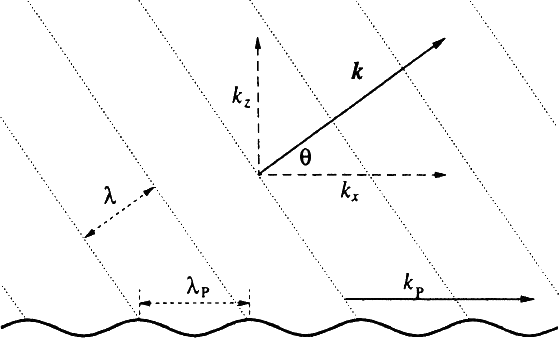
\includegraphics[width=0.7\linewidth]{00_Images/05_chapter/08.png}
    \caption{Wavevector matching and radiation angle for large vibrating plates}
    \label{fig:plate_radiation_angle}
\end{figure}
